\section{Standard Method in Itemset Mining}

After encoding the base constraints,
we proceed to employ the standard method to encode formula \ref{eq:4}.

To solve the problem $q_1 + q_2 + ... + q_n \ge \lambda$, we can use the standard method known as $C_{n-k+1}$.

The algorithm's idea is as follows: Suppose we have a set of $n$ elements.
If there are at least $k$ true elements, it is equivalent to having at most $n-k$ false elements.
In other words, when selecting $n-k+1$ elements, we are guaranteed to have at least one true element among them.

% image
\begin{figure}[H]
    \centering
    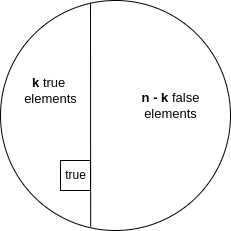
\includegraphics[width=0.38\textwidth]{chapter2/image/standard.png}
    \caption{Illustration of the standard method $C_{n-k+1}$}
    \label{fig:2_1}
\end{figure}

For example, suppose $n = 5$ and $\lambda = 3$, we can use the constraint below to represent the concept of having at least 3 true elements among 5 elements.
\begin{equation}
    \label{eq:5}
    \begin{aligned}
               & (q_1 \vee q_2 \vee q_3) \\
        \wedge & (q_1 \vee q_2 \vee q_4) \\
        \wedge & (q_1 \vee q_2 \vee q_5) \\
        \wedge & (q_1 \vee q_3 \vee q_4) \\
        \wedge & (q_1 \vee q_3 \vee q_5) \\
        \wedge & (q_1 \vee q_4 \vee q_5) \\
        \wedge & (q_2 \vee q_3 \vee q_4) \\
        \wedge & (q_2 \vee q_3 \vee q_5) \\
        \wedge & (q_2 \vee q_4 \vee q_5) \\
        \wedge & (q_3 \vee q_4 \vee q_5) \\
    \end{aligned}
\end{equation}

Then with $n$ elements and $\lambda$, we can present the constraint as:
\begin{equation}
    \label{eq:6}
    \begin{aligned}
         & \bigwedge_{i=1}^{n-\lambda+1} \left( \bigvee_{j=i}^{i+\lambda-1} q_j \right) \\
    \end{aligned}
\end{equation}

Now, we can use constraints \ref{eq:2}, \ref{eq:3} and \ref{eq:6} to resolve the problem Itemset Mining.